\chapter{Лекция}
\label{ch:intro}

\section*{Что такое SDR?}

\textbf{Software-Defined Radio (SDR)} - радиосистема, в которой часть аппаратных компонентов (фильтры, модуляторы и т.п.) 
реализованы на программном уровне.

\section*{Базовая архитектура системы радиосвязи}

\begin{figure}[H]
    \centering
    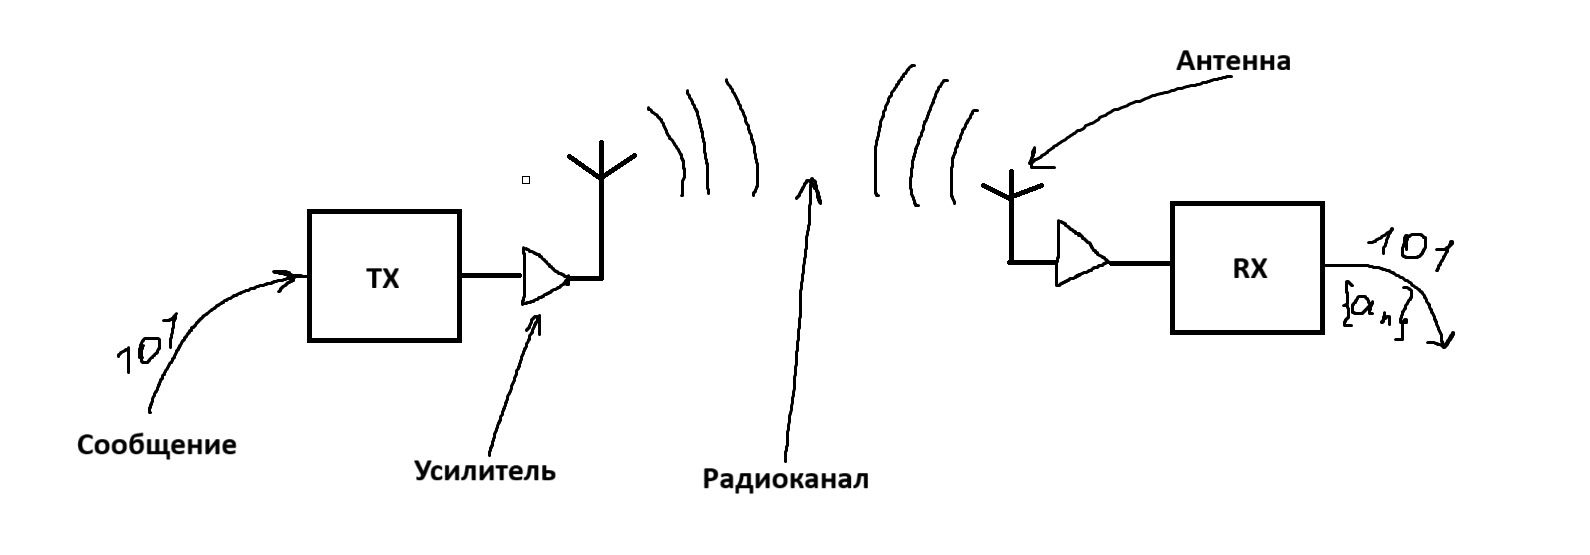
\includegraphics[width=1.0\textwidth]{base_arch.png}
    \caption{Архитектура системы радиосвязи в целом}
\end{figure}

\section*{Описание компонентов архитектуры}

Базовая архитектура состоит из \textbf{передатчика (TX)} и \textbf{приемника (RX)}. Между ними находится \textbf{радиоканал - среда}, в которой распространяется сигнал. У \textbf{TX} и \textbf{RX} есть \textbf{антенна - устройство}, которое излучает или принимает электромагнитные волны, и преобразует их в электрический ток и обратно, в самом простом случае это просто кусок проволоки. Также и у \textbf{TX} и у \textbf{RX} есть \textbf{усилитель}, который усиливает отправляемый/принимаемый сигнал.

\section*{Описание процесса обмена данными}

На стороне \textbf{TX} формируется \textbf{сообщение}, которое необходимо передать. Это сообщение поступает в передатчик в виде набора \textbf{нулей и единиц}. \textbf{TX} преобразует нули и единицы определенным образом в электрические колебания, которые через \textbf{антенну} излучаются в виде электромагнитных колебаний в радиоканал.\\
В этом же радиоканале находится \textbf{приемник}, \textbf{антенна} которого принимает эти электромагнитные колебания и преобразует в электрический ток. После этого электрические колебания определенным образом преобразуется в набор нулей и единиц (сообщение, которое отправлял \textbf{TX}). Стоит отметить, что \textbf{прием сообщения} намного сложнее, чем отправка. Это связано с изменениями, которым подвергается сигнал во время прохождения через \textbf{радиоканал}. Сигнал изменяется случайным образом, поэтому точно сказать, как изменится сигнал, мы не можем, мы можем это только предположить с какой-то точностью. Эта проблема решается путем добавления в исходный сигнал \textbf{избыточности}, которая позволяет с более высокой точностью принять сигнал на стороне приемника. Такой избыточностью может быть \textbf{контрольная сумма - число}, которое вычисляется по определенному алгоритму, который учитывает позицию бита и его значение, т.е если хоть в какой нибудь позиции изменится значение бита, то \textbf{контрольная сумма} будет уже другой, что сигнализирует об искажении сигнала.

\section*{Внутренняя архитектура TX}

\begin{figure}[H]
    \centering
    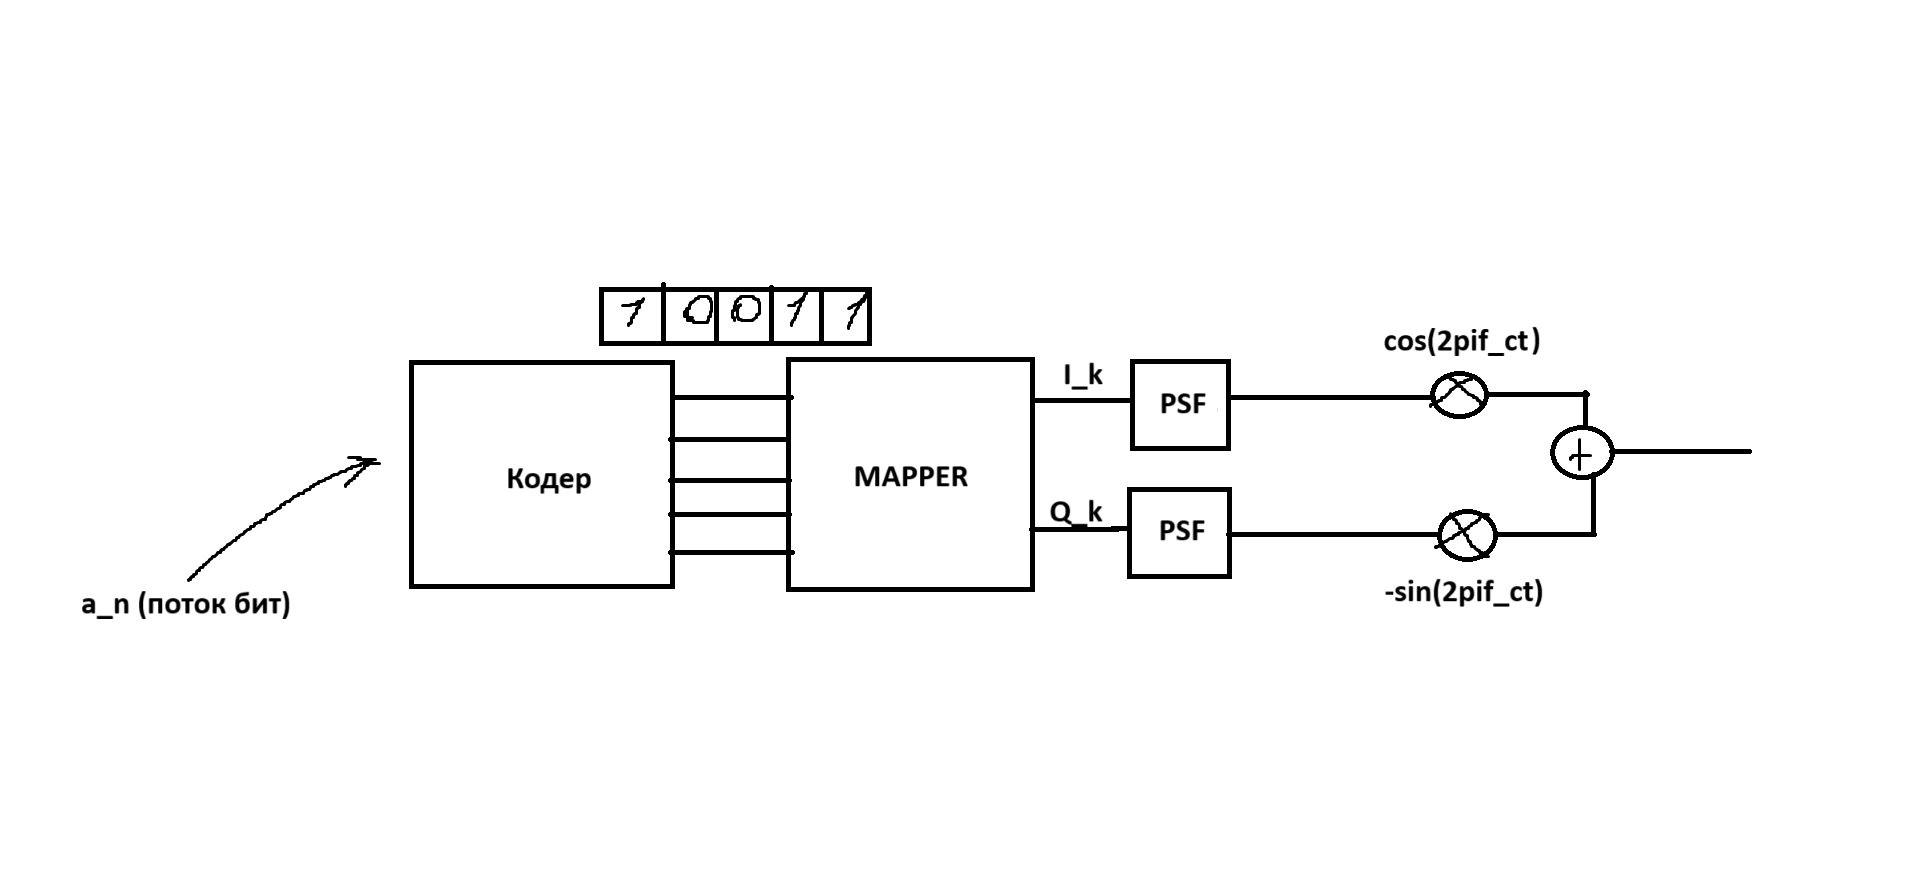
\includegraphics[width=1.0\textwidth]{tx_arch.png}
    \caption{TX архитектура}
\end{figure}

\section*{Coder}
В нашем случае кодер будет выполнять единственную задачу - формировать из потока бит блоки (допустим по 8 бит) и
направлять их в Mapper.

\section*{Mapper}

Устройство, выполняющее \textbf{отображение исходных данных на множество символов или сигналов} в соответствии с выбранной схемой модуляции. 

\medskip

Символ - элемент сиганльного множества. \\

Сигнальное множество - набор состояний радиосигнала. \\

Иными словами: mapper берет блок битов (у нас это 8 бит) и сопоставляет его сигналу с определенными характеристиками, для 
этого в mapper хранится таблица с комбинациями битов и соответсвующие им символы. Если в блоке
8 бит, то всего должно быть 256 символов (на каждую возможную комбинацию). \\

\begin{figure}[H]
    \centering
    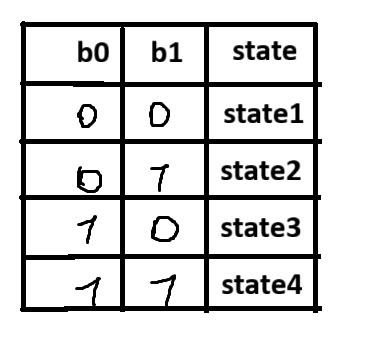
\includegraphics[width=1.0\textwidth]{mapper_table.png}
    \caption{Пример таблицы в маппере}
\end{figure}

Также для визуализации данного процесса используется созвездие символов \\

\textbf{Созвездие символов} - это \textbf{графическое представление множества возможных символов модуляции} в комплексной плоскости.  
Каждый символ соответствует определённой комбинации параметров сигнала и изображается в виде точки на диаграмме.  

\begin{figure}[H]
    \centering
    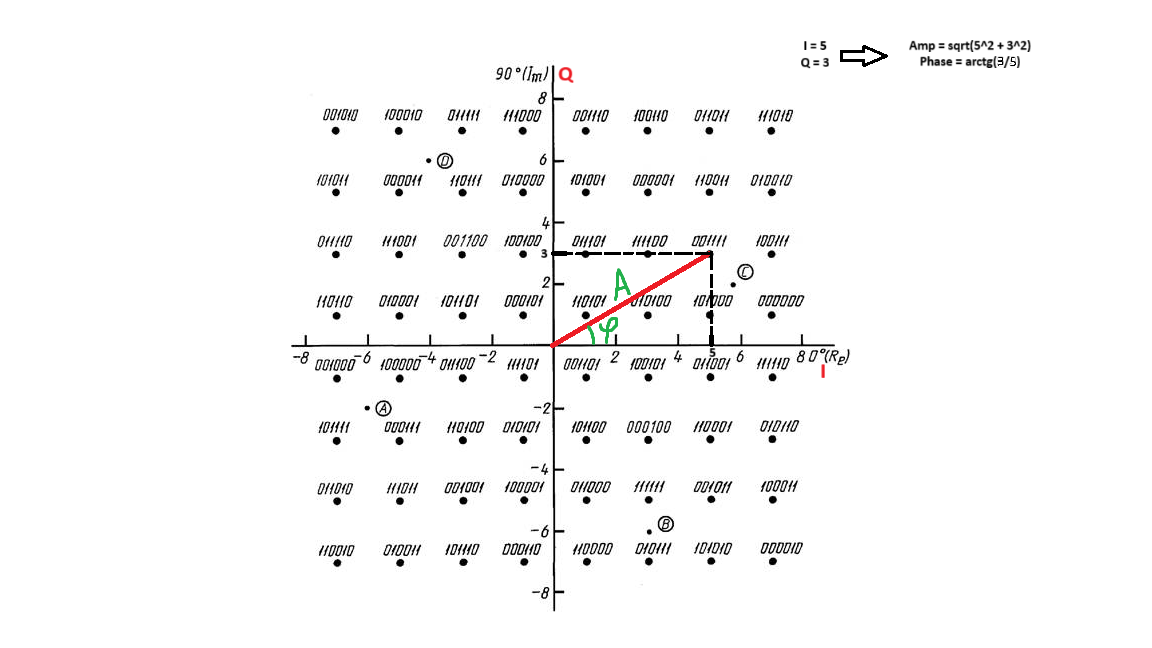
\includegraphics[width=1.0\textwidth]{QAM64.png}
    \caption{Пример созвездия символов}
\end{figure}

Каждой точке соответствуют координаты (I, Q), где I - действительная составляющая, Q - мнимая. Зная координаты, можем вычислить
длину радиус-вектора до этой точки, это будет амплитудой этого сигнала, угол между действительной осью и радиус-вектором - фаза
сигнала.

От mapper идет 2 выхода, один для I составляющей, другой для Q составляющей, которые поступают на вход формирующего фильтра.

\section*{Формирующий фильтр}

Устройство, преобразующее последовательности символов в непрерывный сигнал с заданной формой. Этот фильтр должен превратить символы (I и Q) в длительные (передаваемые) символы (символы, растянутые по по времени с длиной $T_s$)

\begin{figure}[H]
    \centering
    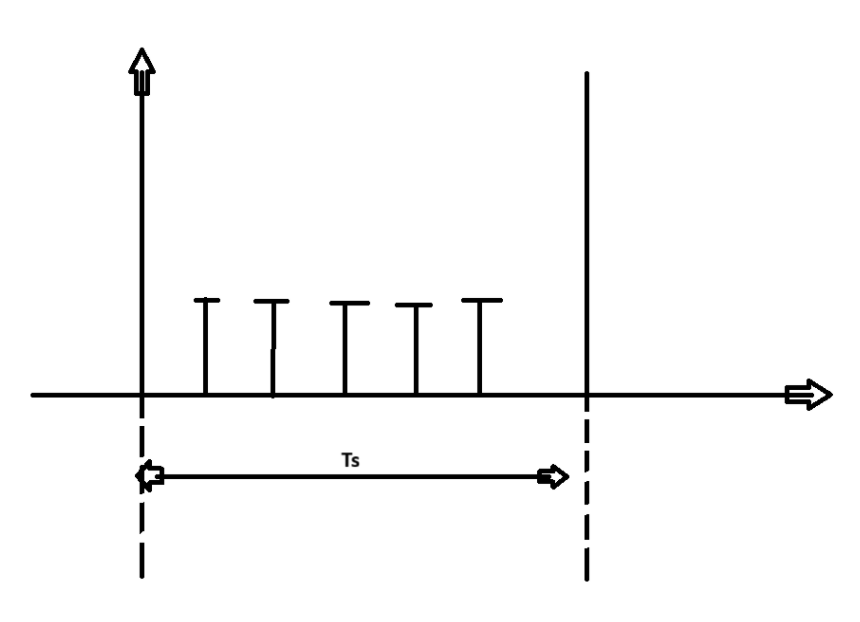
\includegraphics[width=1.0\textwidth]{pulse.png}
    \caption{Пример длительного символа}
\end{figure}

До этого момента все выполнялось программно. Всё, что будет дальше - работа самой SDR. \\

Далее происходит генерация непрерывного сигнала. Математически этот процесс можно записать
следующим образом:

$$s(t) = I(t)\cos(2\pi f_c t) - Q(t)\sin(2\pi f_c t)$$

$f_c$ здесь - несущая частота (высокочастотное колебание).

\endinput